% Created 2014-08-27 mié 09:12
\documentclass[xcolor={usenames,svgnames,dvipsnames}]{beamer}
\usepackage[utf8]{inputenc}
\usepackage[T1]{fontenc}
\usepackage{fixltx2e}
\usepackage{graphicx}
\usepackage{longtable}
\usepackage{float}
\usepackage{wrapfig}
\usepackage{rotating}
\usepackage[normalem]{ulem}
\usepackage{amsmath}
\usepackage{textcomp}
\usepackage{marvosym}
\usepackage{wasysym}
\usepackage{amssymb}
\usepackage{hyperref}
\tolerance=1000
\usepackage{color}
\usepackage{listings}
\AtBeginSection[]{\begin{frame}[plain]\tableofcontents[currentsection,hideallsubsections]\end{frame}}
\lstset{keywordstyle=\color{blue}, commentstyle=\color{gray!90}, basicstyle=\ttfamily\small, columns=fullflexible, breaklines=true,linewidth=\textwidth, backgroundcolor=\color{gray!23}, basewidth={0.5em,0.4em}, literate={á}{{\'a}}1 {ñ}{{\~n}}1 {é}{{\'e}}1 {ó}{{\'o}}1 {º}{{\textordmasculine}}1}
\usepackage{mathpazo}
\hypersetup{colorlinks=true, linkcolor=Blue, urlcolor=Blue}
\usepackage{fancyvrb}
\DefineVerbatimEnvironment{verbatim}{Verbatim}{fontsize=\tiny, formatcom = {\color{black!70}}}
\usetheme{Goettingen}
\usecolortheme{rose}
\usefonttheme{serif}
\author{Oscar Perpiñán Lamigueiro \\ \url{http://oscarperpinan.github.io}}
\date{}
\title{Gráficos con R}
\hypersetup{
  pdfkeywords={},
  pdfsubject={},
  pdfcreator={Emacs 24.3.1 (Org mode 8.2.1)}}
\begin{document}

\maketitle


\section{Introducción}
\label{sec-1}
\subsection{Base y grid}
\label{sec-1-1}
\begin{frame}[fragile,label=sec-1-1-1]{Base y grid}
 En \texttt{R} existen dos formas de generar gráficos:
\begin{itemize}
\item Base graphics
\item Grid graphics
\end{itemize}

Dentro del conjunto \texttt{grid} existen dos grandes paquetes:
\begin{itemize}
\item \texttt{lattice}
\item \texttt{ggplot2}
\end{itemize}
\end{frame}
\begin{frame}[fragile,label=sec-1-1-2]{Conjunto de datos de ejemplo}
 \begin{itemize}
\item Leemos desde el archivo local
\end{itemize}
\lstset{language=R,numbers=none}
\begin{lstlisting}
aranjuez <- read.csv('data/aranjuez.csv')

summary(aranjuez)
\end{lstlisting}

\begin{verbatim}
         X           TempAvg          TempMax          TempMin       
2004-01-01:   1   Min.   :-5.309   Min.   :-2.362   Min.   :-12.980  
2004-01-02:   1   1st Qu.: 7.692   1st Qu.:14.530   1st Qu.:  1.515  
2004-01-03:   1   Median :13.810   Median :21.670   Median :  7.170  
2004-01-04:   1   Mean   :14.405   Mean   :22.531   Mean   :  6.888  
2004-01-05:   1   3rd Qu.:21.615   3rd Qu.:30.875   3rd Qu.: 12.590  
2004-01-06:   1   Max.   :30.680   Max.   :41.910   Max.   : 22.710  
(Other)   :2892                                     NA's   :4        
   HumidAvg         HumidMax         WindAvg         WindMax      
Min.   : 19.89   Min.   : 35.88   Min.   :0.251   Min.   : 0.000  
1st Qu.: 47.04   1st Qu.: 81.60   1st Qu.:0.667   1st Qu.: 3.783  
Median : 62.58   Median : 90.90   Median :0.920   Median : 5.027  
Mean   : 62.16   Mean   : 87.22   Mean   :1.174   Mean   : 5.208  
3rd Qu.: 77.38   3rd Qu.: 94.90   3rd Qu.:1.431   3rd Qu.: 6.537  
Max.   :100.00   Max.   :100.00   Max.   :8.260   Max.   :10.000  
                 NA's   :13       NA's   :8       NA's   :128     
     Rain          Radiation            ET       
Min.   : 0.000   Min.   : 0.277   Min.   :0.000  
1st Qu.: 0.000   1st Qu.: 9.370   1st Qu.:1.168  
Median : 0.000   Median :16.660   Median :2.758  
Mean   : 1.094   Mean   :16.742   Mean   :3.091  
3rd Qu.: 0.200   3rd Qu.:24.650   3rd Qu.:4.926  
Max.   :49.730   Max.   :32.740   Max.   :8.564  
NA's   :4        NA's   :13       NA's   :18
\end{verbatim}
\end{frame}
\begin{frame}[fragile,label=sec-1-1-3]{Conjunto de datos de ejemplo}
 \begin{itemize}
\item Añadimos algunas columnas
\end{itemize}
\lstset{language=R,numbers=none}
\begin{lstlisting}
aranjuez$month <- as.numeric(
		  format(as.Date(aranjuez$X), '%m'))
aranjuez$year <- as.numeric(
		 format(as.Date(aranjuez$X), '%Y'))
aranjuez$day <- as.numeric(
		format(as.Date(aranjuez$X), '%j'))
aranjuez$jday <- julian(as.Date(aranjuez$X))
aranjuez$quarter <- quarters(as.Date(aranjuez$X))
\end{lstlisting}
\end{frame}

\section{Grid}
\label{sec-2}

\subsection{Lattice}
\label{sec-2-1}

\begin{frame}[fragile,label=sec-2-1-1]{Lattice}
 \begin{itemize}
\item Documentación: \href{http://lmdvr.r-forge.r-project.org/figures/figures.html}{Código y Figuras del libro}
\end{itemize}

\lstset{language=R,numbers=none}
\begin{lstlisting}
library(lattice)
\end{lstlisting}
\end{frame}
\begin{frame}[fragile,label=sec-2-1-2]{\texttt{xyplot}}
 \lstset{language=R,numbers=none}
\begin{lstlisting}
xyplot(Radiation ~ TempAvg, data=aranjuez)
\end{lstlisting}

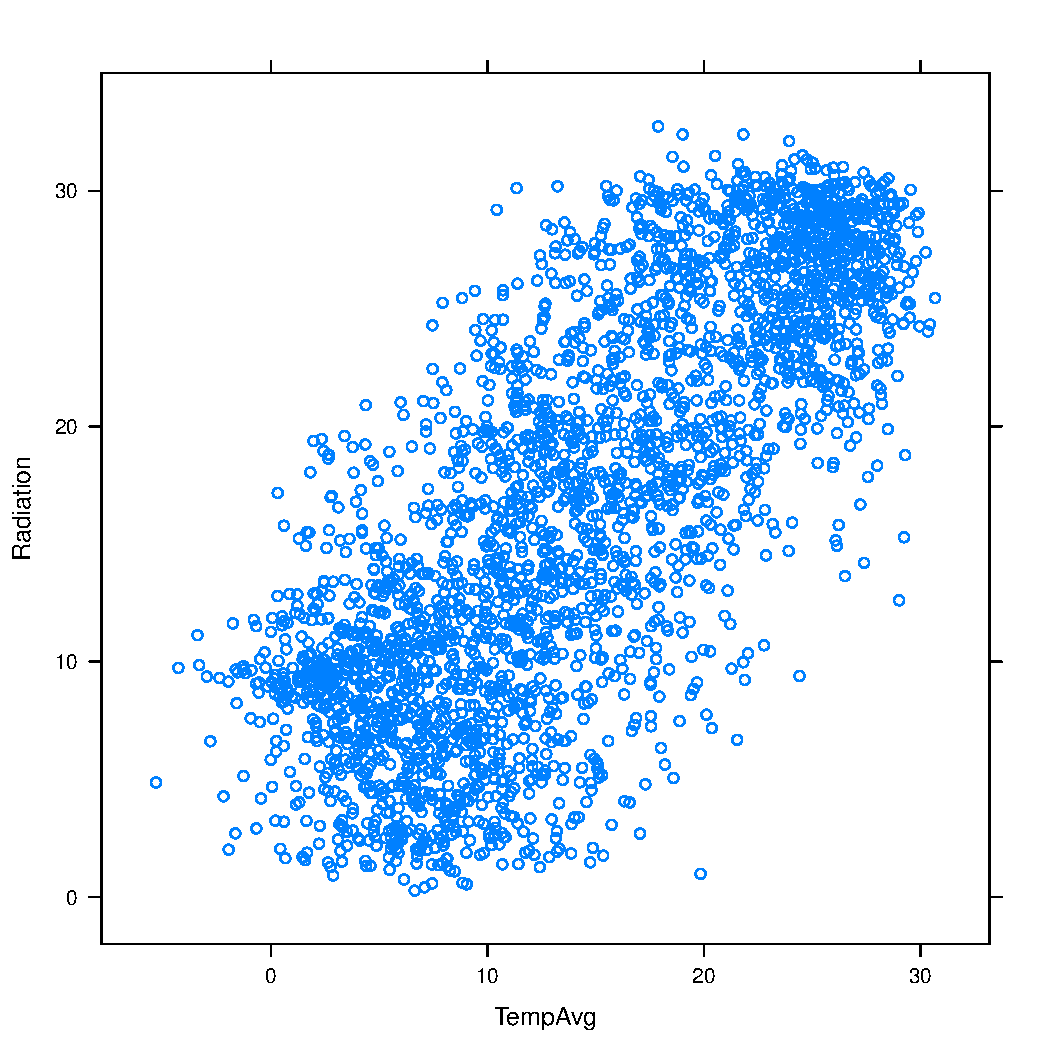
\includegraphics[width=.9\linewidth]{figs/xyplot.pdf}
\end{frame}

\begin{frame}[fragile,label=sec-2-1-3]{\texttt{xyplot}}
 \lstset{language=R,numbers=none}
\begin{lstlisting}
xyplot(Radiation ~ TempAvg, data=aranjuez,
       type=c('p', 'g'))
\end{lstlisting}

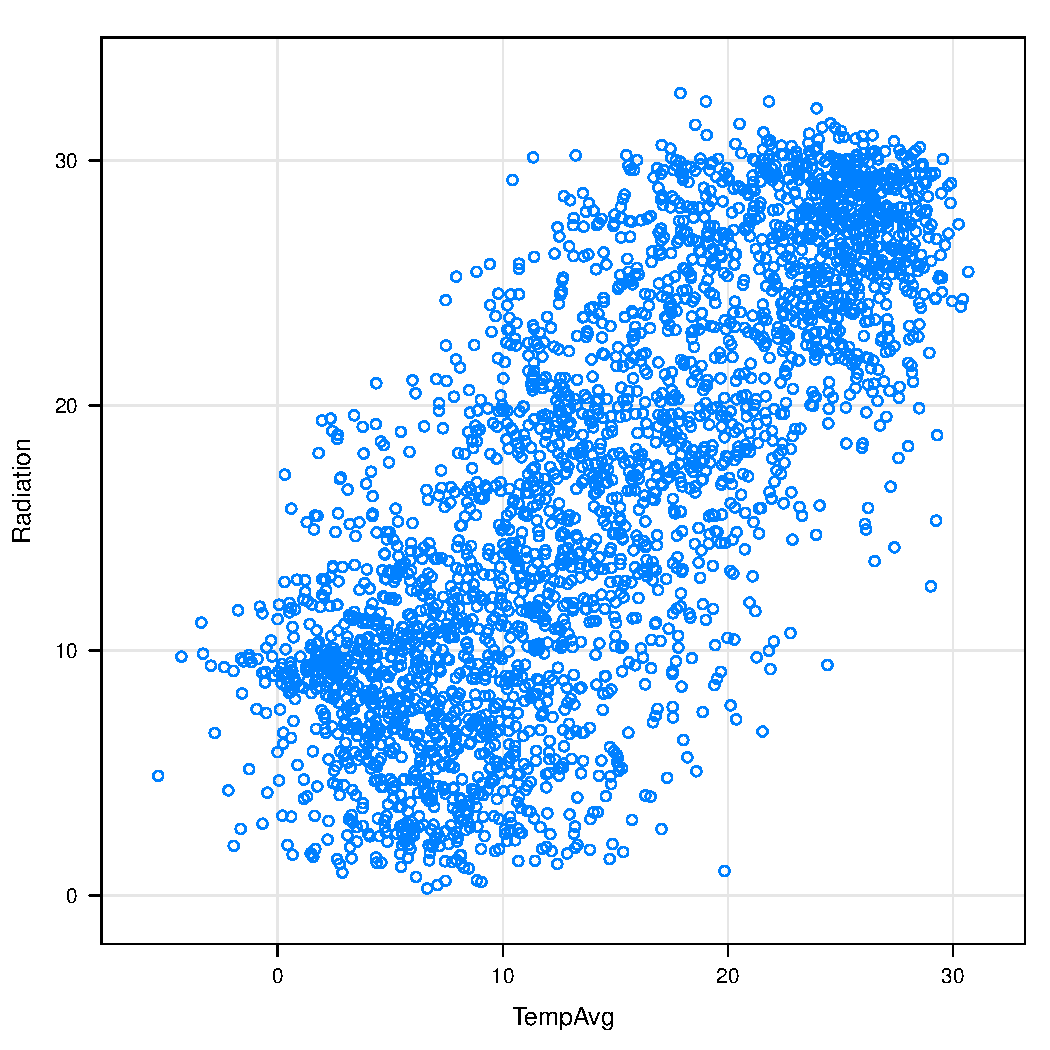
\includegraphics[width=.9\linewidth]{figs/xyplotPG.pdf}
\end{frame}

\begin{frame}[fragile,label=sec-2-1-4]{\texttt{xyplot}}
 \lstset{language=R,numbers=none}
\begin{lstlisting}
xyplot(Radiation ~ TempAvg, data=aranjuez,
       type=c('p', 'r', 'g'),
       lwd=2, col.line='black')
\end{lstlisting}

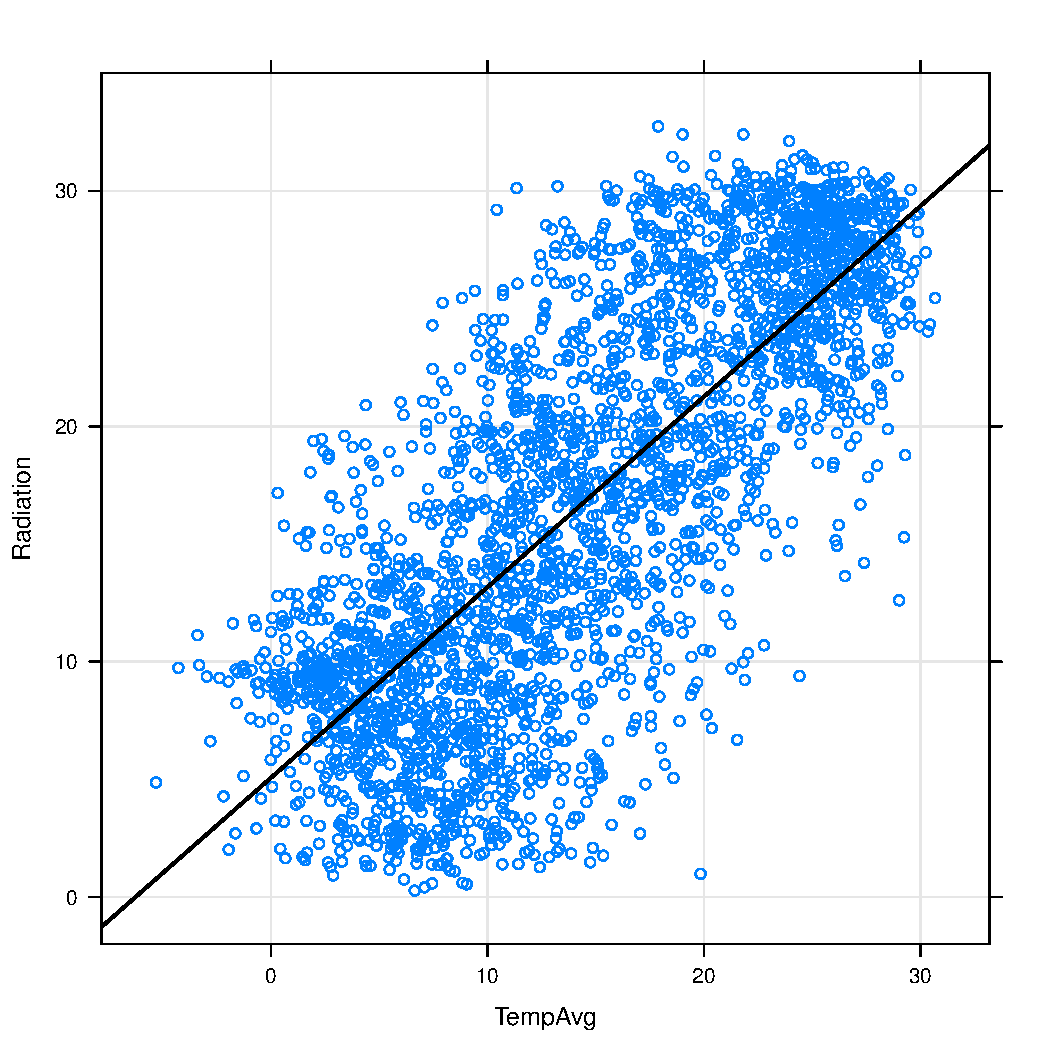
\includegraphics[width=.9\linewidth]{figs/xyplotPRG.pdf}
\end{frame}

\begin{frame}[fragile,label=sec-2-1-5]{\texttt{xyplot}}
 \lstset{language=R,numbers=none}
\begin{lstlisting}
xyplot(Radiation ~ TempAvg, data=aranjuez,
       type=c('p', 'smooth', 'g'),
       lwd=2, col.line='black')
\end{lstlisting}

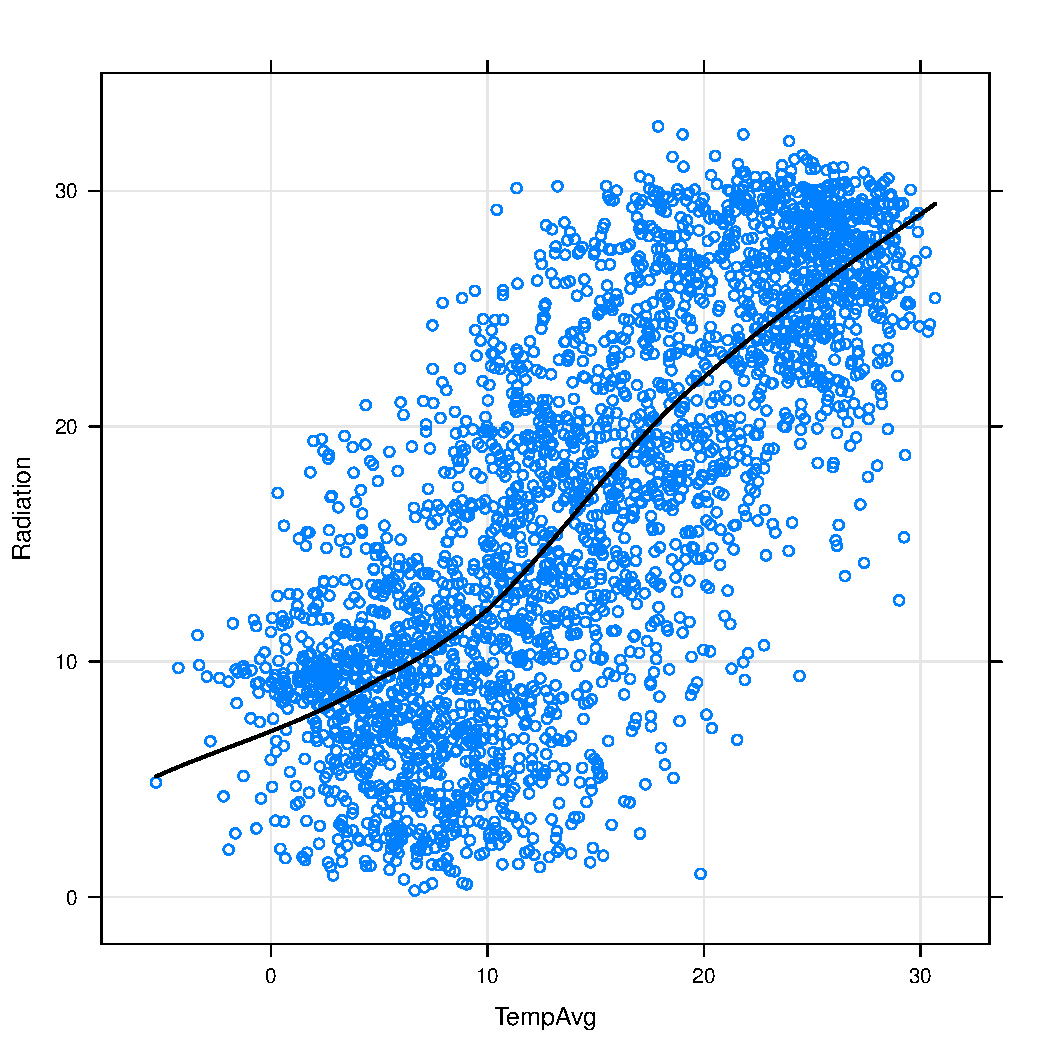
\includegraphics[width=.9\linewidth]{figs/xyplotSmooth.pdf}
\end{frame}

\begin{frame}[fragile,label=sec-2-1-6]{Paneles}
 \lstset{language=R,numbers=none}
\begin{lstlisting}
xyplot(Radiation ~ TempAvg|factor(year),
       data=aranjuez)
\end{lstlisting}

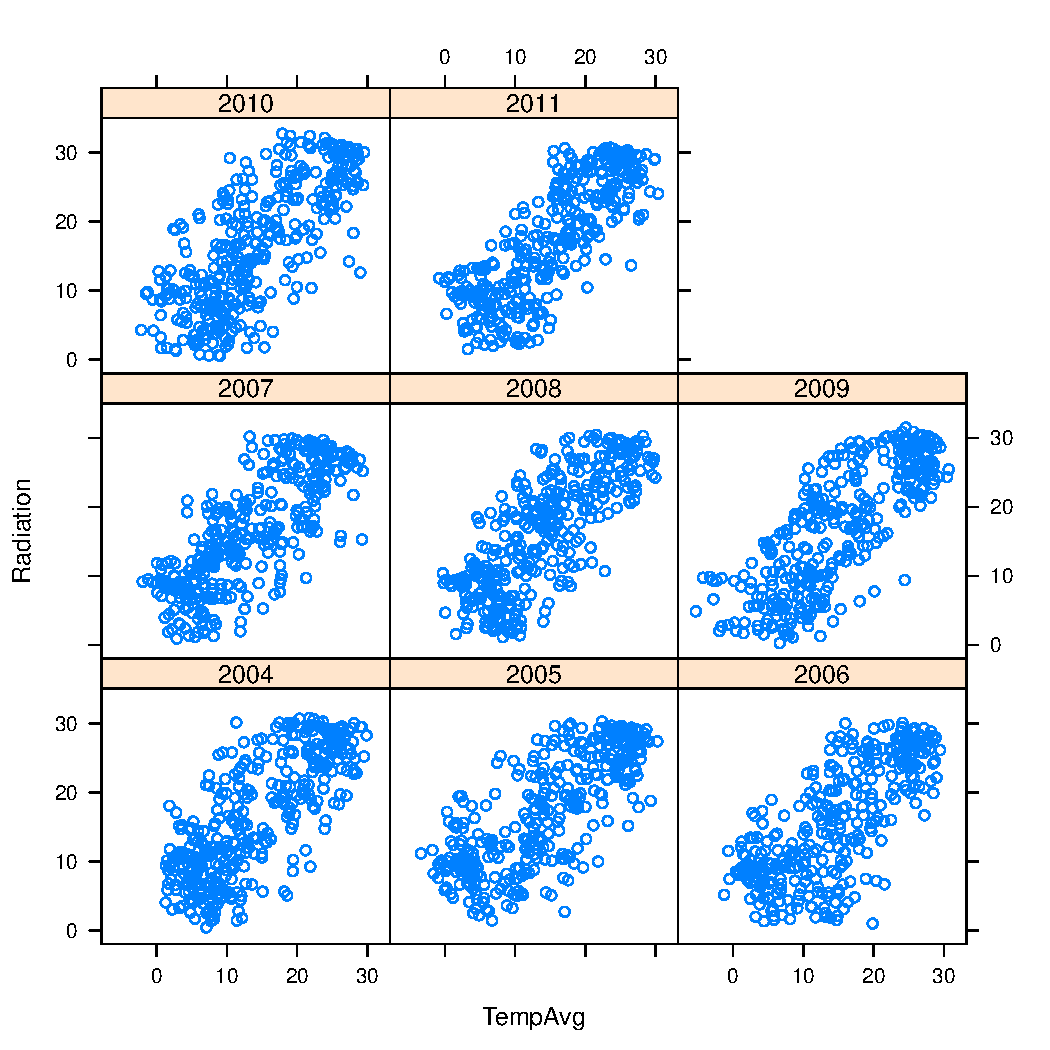
\includegraphics[width=.9\linewidth]{figs/xyplotYear.pdf}
\end{frame}
\begin{frame}[fragile,label=sec-2-1-7]{Grupos}
 \lstset{language=R,numbers=none}
\begin{lstlisting}
xyplot(Radiation ~ TempAvg, groups=quarter,
       data=aranjuez, auto.key=list(space='right'))
\end{lstlisting}

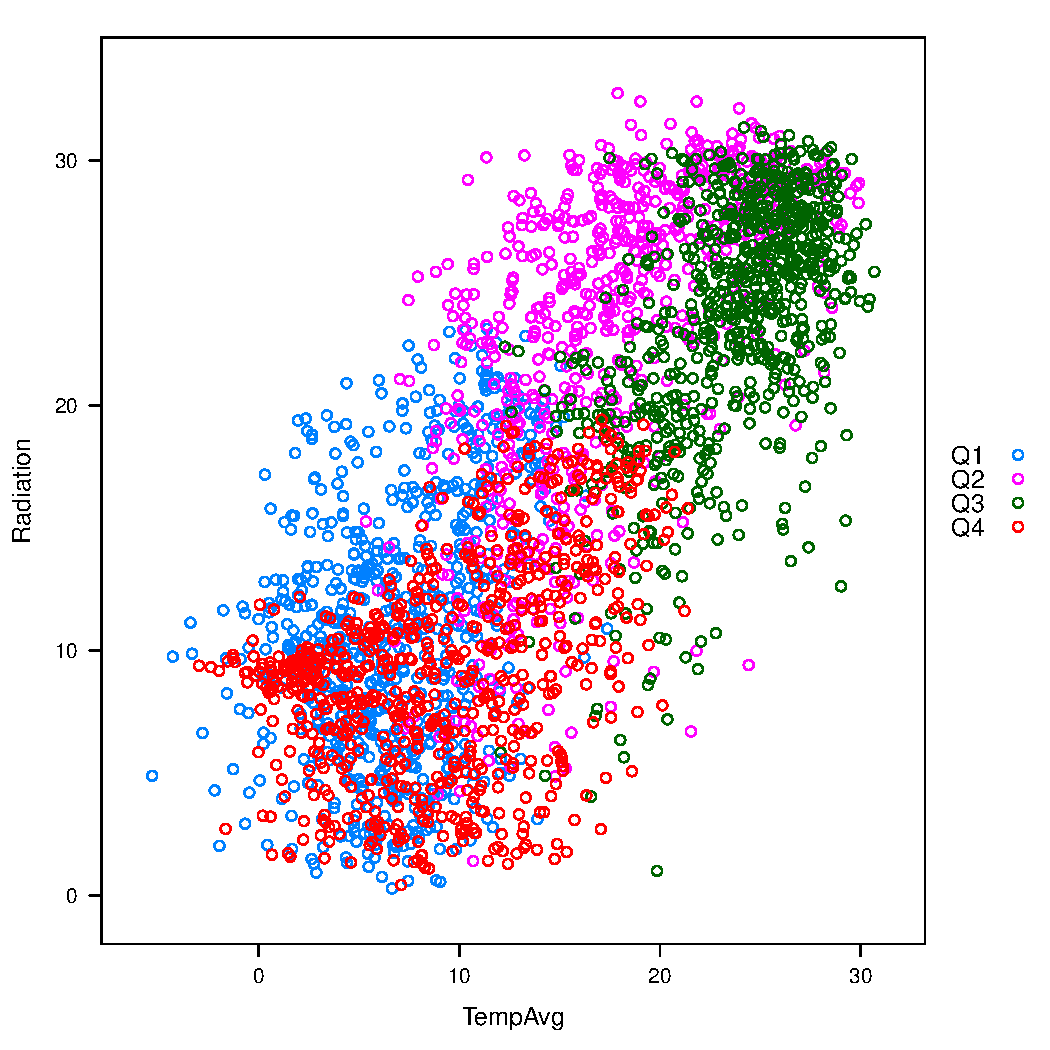
\includegraphics[width=.9\linewidth]{figs/xyplotQuarter.pdf}
\end{frame}
\begin{frame}[fragile,label=sec-2-1-8]{Paneles y grupos}
 \lstset{language=R,numbers=none}
\begin{lstlisting}
xyplot(Radiation ~ TempAvg|factor(year),
       groups=quarter,
       data=aranjuez,
       layout=c(4, 2),
       auto.key=list(space='right'))
\end{lstlisting}

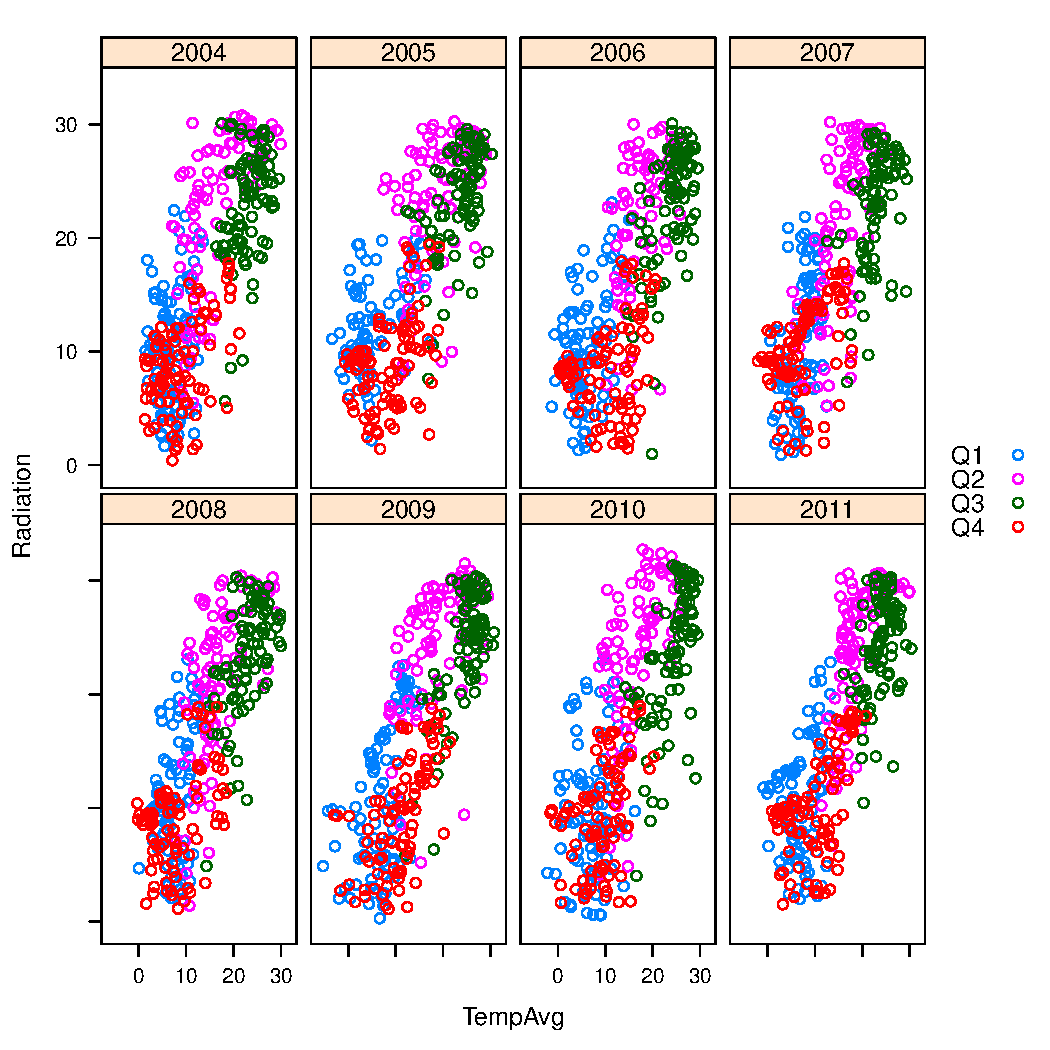
\includegraphics[width=.9\linewidth]{figs/xyplotQuarterYear.pdf}
\end{frame}
\begin{frame}[fragile,label=sec-2-1-9]{Paneles y grupos}
 \lstset{language=R,numbers=none}
\begin{lstlisting}
xyplot(Radiation ~ TempAvg|factor(year),
       groups=quarter,
       data=aranjuez,
       layout=c(4, 2),
       type=c('p', 'r'),
       auto.key=list(space='right'))
\end{lstlisting}

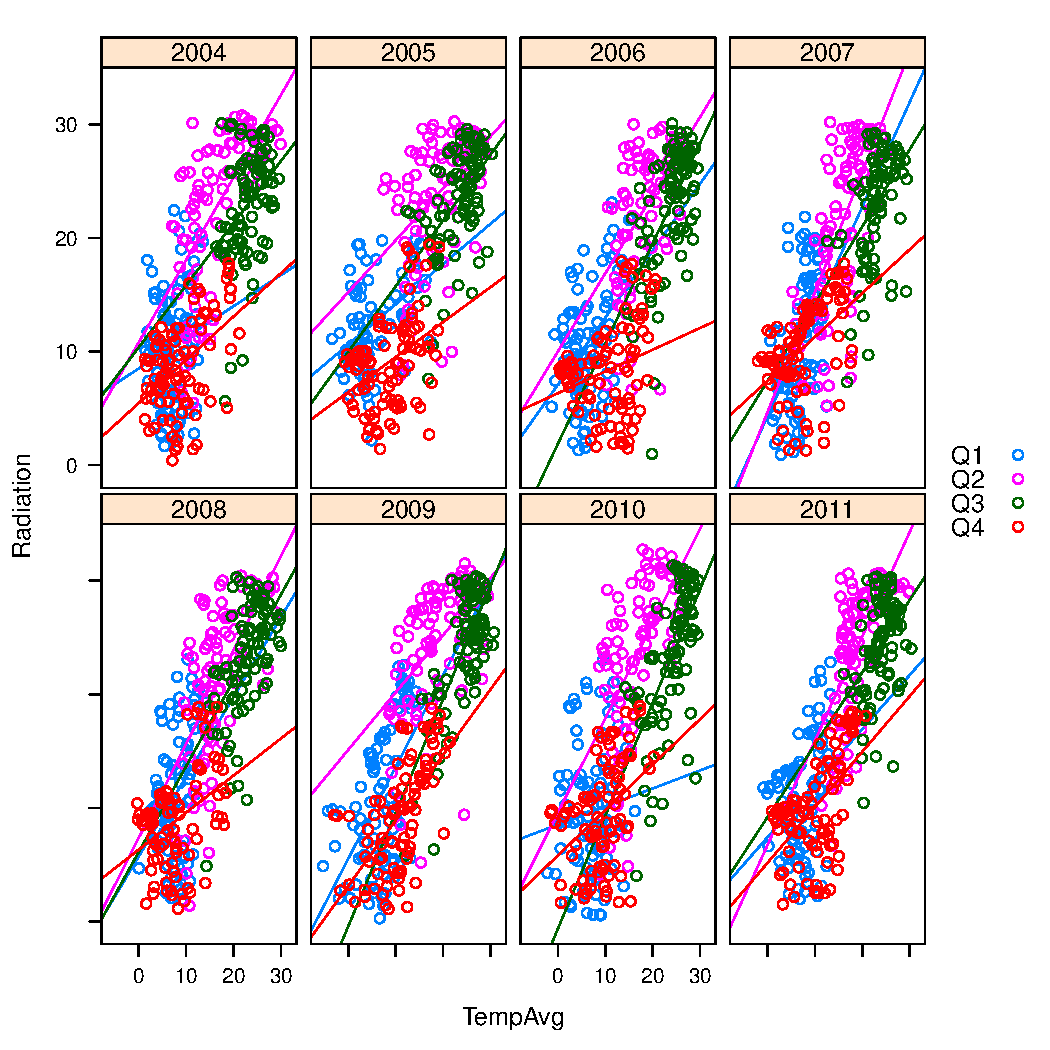
\includegraphics[width=.9\linewidth]{figs/xyplotQuarterYearSmooth.pdf}
\end{frame}
\begin{frame}[fragile,label=sec-2-1-10]{Colores y tamaños}
 \lstset{language=R,numbers=none}
\begin{lstlisting}
xyplot(Radiation ~ TempAvg,
       type=c('p', 'r'),
       cex=2, col='blue',
       alpha=.5, pch=19,
       lwd=3, col.line='black',
       data=aranjuez)
\end{lstlisting}

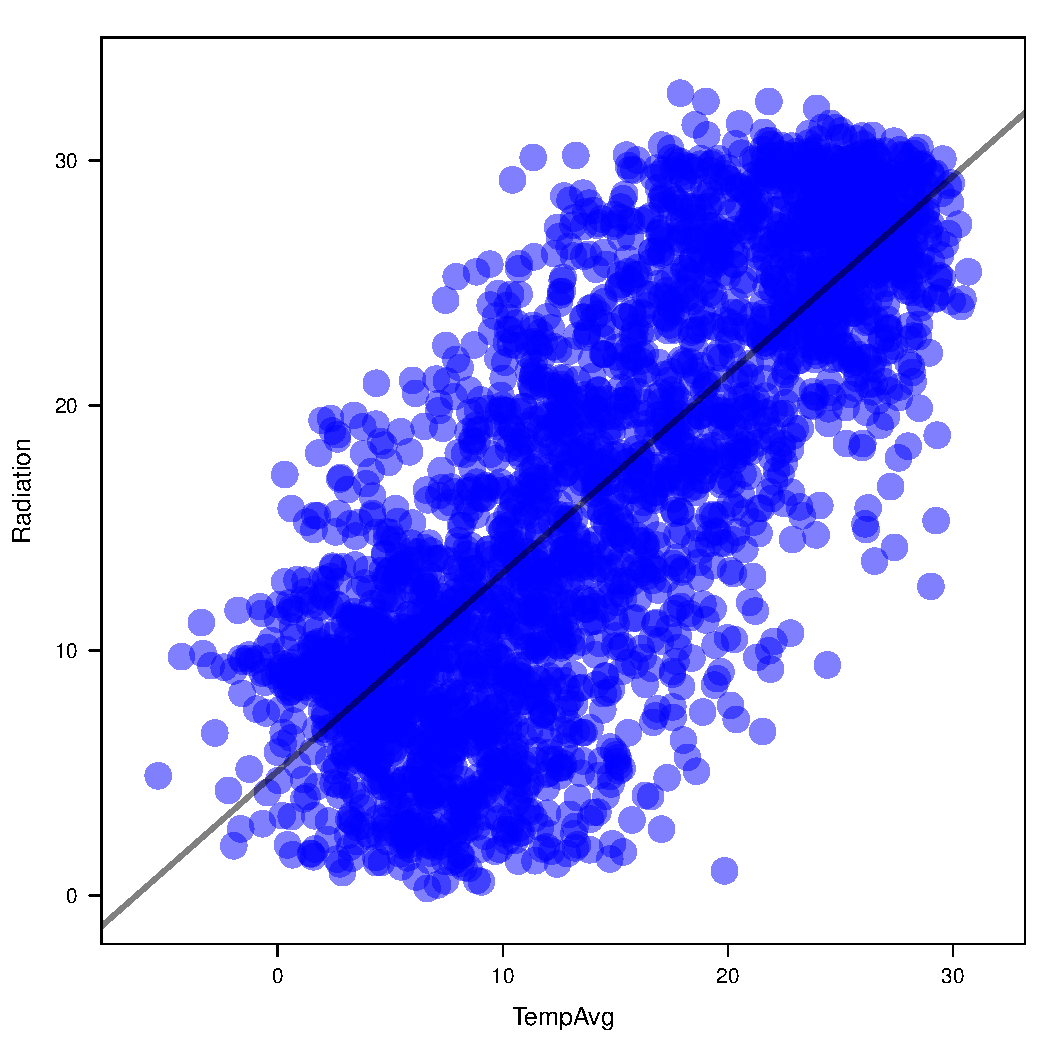
\includegraphics[width=.9\linewidth]{figs/xyplotColors.pdf}
\end{frame}
\begin{frame}[fragile,label=sec-2-1-11]{Colores con grupos}
 \lstset{language=R,numbers=none}
\begin{lstlisting}
xyplot(Radiation ~ TempAvg,
       group=quarter,
       col=c('red', 'blue', 'green', 'yellow'),
       pch=19,
       auto.key=list(space='right'),
       data=aranjuez)
\end{lstlisting}

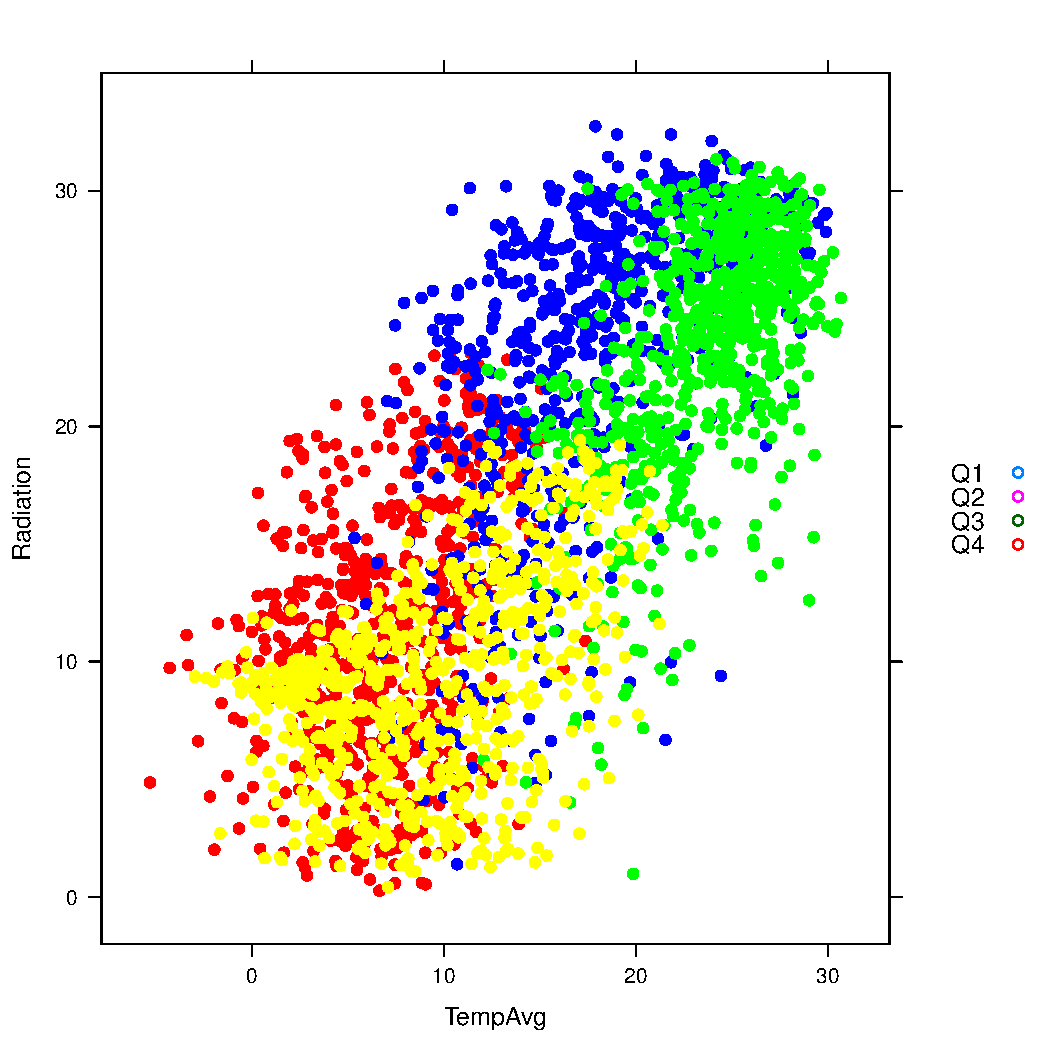
\includegraphics[width=.9\linewidth]{figs/xyplotColorGroups.pdf}
\end{frame}
\begin{frame}[fragile,label=sec-2-1-12]{Colores con grupos: \texttt{par.settings} y \texttt{simpleTheme}}
 \begin{itemize}
\item Primero definimos el tema con \texttt{simpleTheme}
\end{itemize}
\lstset{language=R,numbers=none}
\begin{lstlisting}
myTheme <- simpleTheme(col=c('red', 'blue',
			'green', 'yellow'),
			pch=19, alpha=.6)
\end{lstlisting}
\end{frame}
\begin{frame}[fragile,label=sec-2-1-13]{Colores con grupos: \texttt{par.settings} y \texttt{simpleTheme}}
 \begin{itemize}
\item Aplicamos el resultado en \texttt{par.settings}
\end{itemize}
\lstset{language=R,numbers=none}
\begin{lstlisting}
xyplot(Radiation ~ TempAvg,
       groups=quarter,
       par.settings=myTheme,
       auto.key=list(space='right'),
       data=aranjuez)
\end{lstlisting}

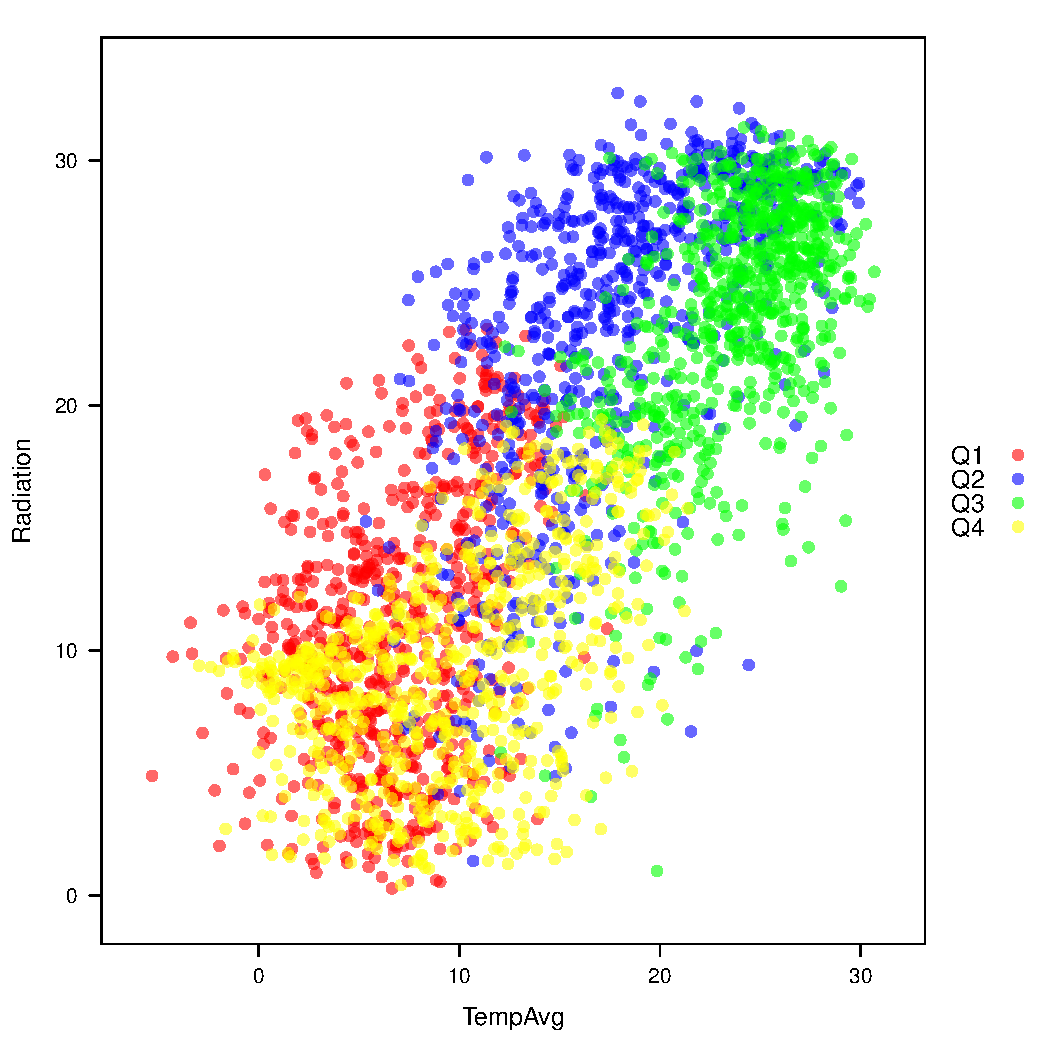
\includegraphics[width=.9\linewidth]{figs/myTheme.pdf}
\end{frame}
\begin{frame}[fragile,label=sec-2-1-14]{Colores: brewer.pal}
 \lstset{language=R,numbers=none}
\begin{lstlisting}
library(RColorBrewer)
myTheme <- custom.theme(symbol=brewer.pal(n=4,
			'Dark2'),
			pch=19, alpha=.6)
xyplot(Radiation ~ TempAvg,
       groups=quarter,
       par.settings=myTheme,
       auto.key=list(space='right'),
       data=aranjuez)
\end{lstlisting}

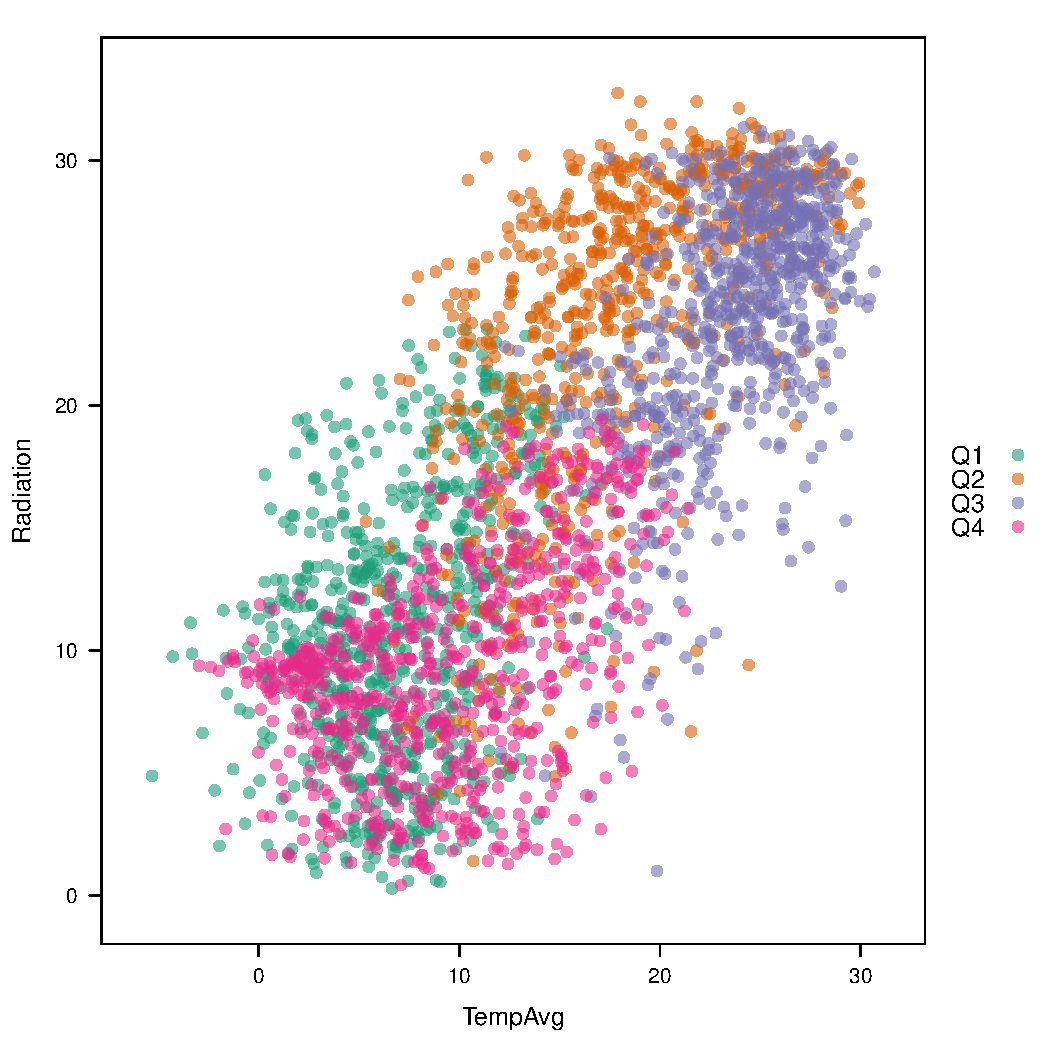
\includegraphics[width=.9\linewidth]{figs/brewer.pdf}
\end{frame}
\begin{frame}[fragile,label=sec-2-1-15]{Paneles a medida}
 \lstset{language=R,numbers=none}
\begin{lstlisting}
xyplot(Radiation ~ TempAvg, data=aranjuez,
       panel=function(x, y, ...){
	   panel.xyplot(x, y, ...)
	   minIdx <- which.min(x)
	   maxIdx <- which.max(x)
	   panel.points(x[c(minIdx, maxIdx)],
			y[c(minIdx, maxIdx)],
			cex=2, col='red')
	   panel.text(x[minIdx], y[minIdx],
		      'MIN', pos=1)
	   })
\end{lstlisting}

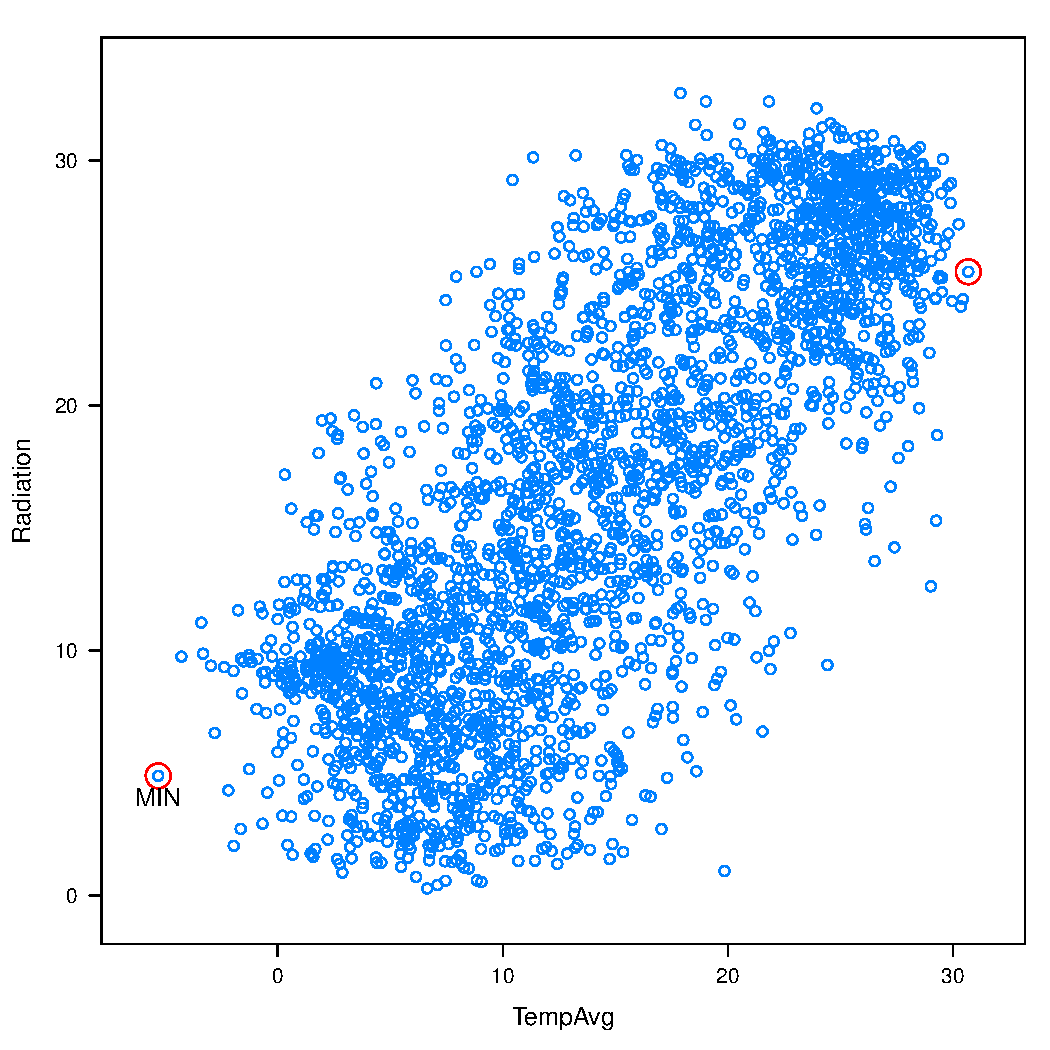
\includegraphics[width=.9\linewidth]{figs/panel.pdf}
\end{frame}
\begin{frame}[fragile,label=sec-2-1-16]{Matriz de gráficos de dispersión}
 \lstset{language=R,numbers=none}
\begin{lstlisting}
splom(aranjuez[,c("TempAvg", "HumidAvg", "WindAvg",
		  "Rain", "Radiation", "ET")],
      pscale=0, alpha=0.6, cex=0.3, pch=19)
\end{lstlisting}

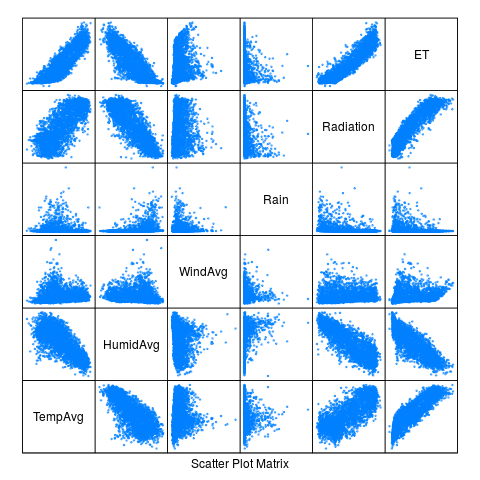
\includegraphics[width=.9\linewidth]{figs/splom.png}
\end{frame}
\begin{frame}[fragile,label=sec-2-1-17]{Matriz de gráficos de dispersión}
 \lstset{language=R,numbers=none}
\begin{lstlisting}
splom(aranjuez[,c("TempAvg", "HumidAvg", "WindAvg",
		  "Rain", "Radiation", "ET")],
      groups=aranjuez$quarter,
      auto.key=list(space='right'),
      pscale=0, alpha=0.6, cex=0.3, pch=19)
\end{lstlisting}

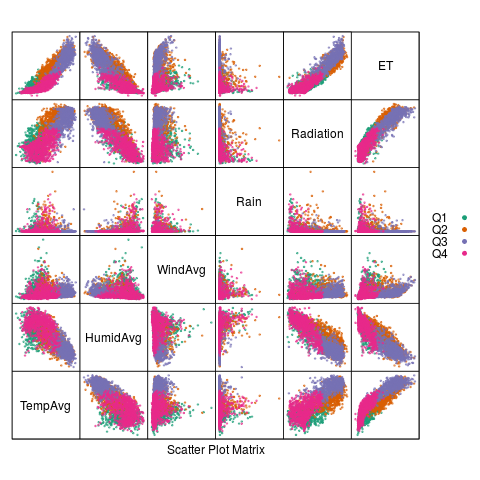
\includegraphics[width=.9\linewidth]{figs/splomGroup.png}
\end{frame}
\begin{frame}[fragile,label=sec-2-1-18]{\texttt{levelplot}}
 \lstset{language=R,numbers=none}
\begin{lstlisting}
levelplot(TempAvg ~ year * day,
	  data=aranjuez)
\end{lstlisting}

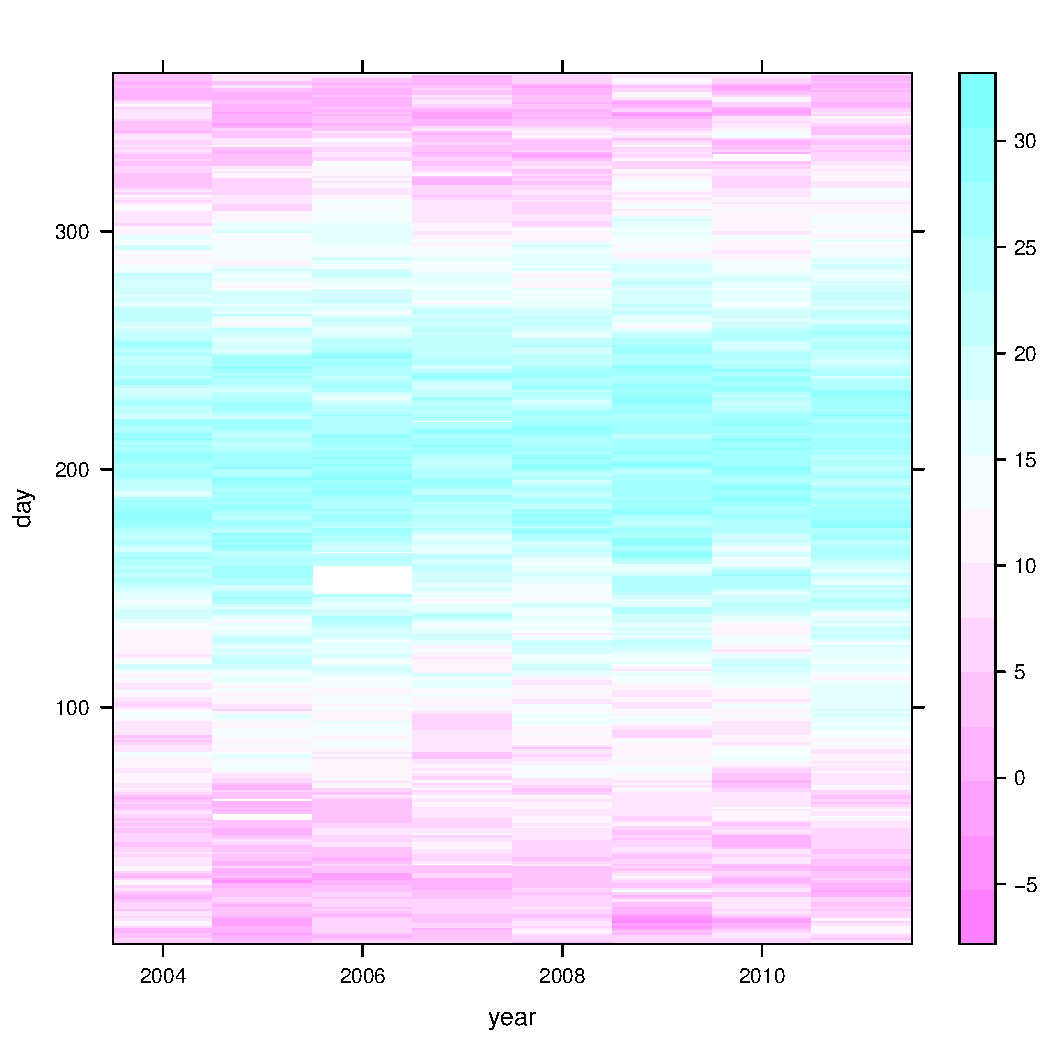
\includegraphics[width=.9\linewidth]{figs/levelplot.pdf}
\end{frame}
\begin{frame}[fragile,label=sec-2-1-19]{\texttt{contourplot}}
 \lstset{language=R,numbers=none}
\begin{lstlisting}
contourplot(Radiation ~ year * day,
	    lwd=.5, labels=FALSE,
	    region=TRUE, 
	    data=aranjuez)
\end{lstlisting}

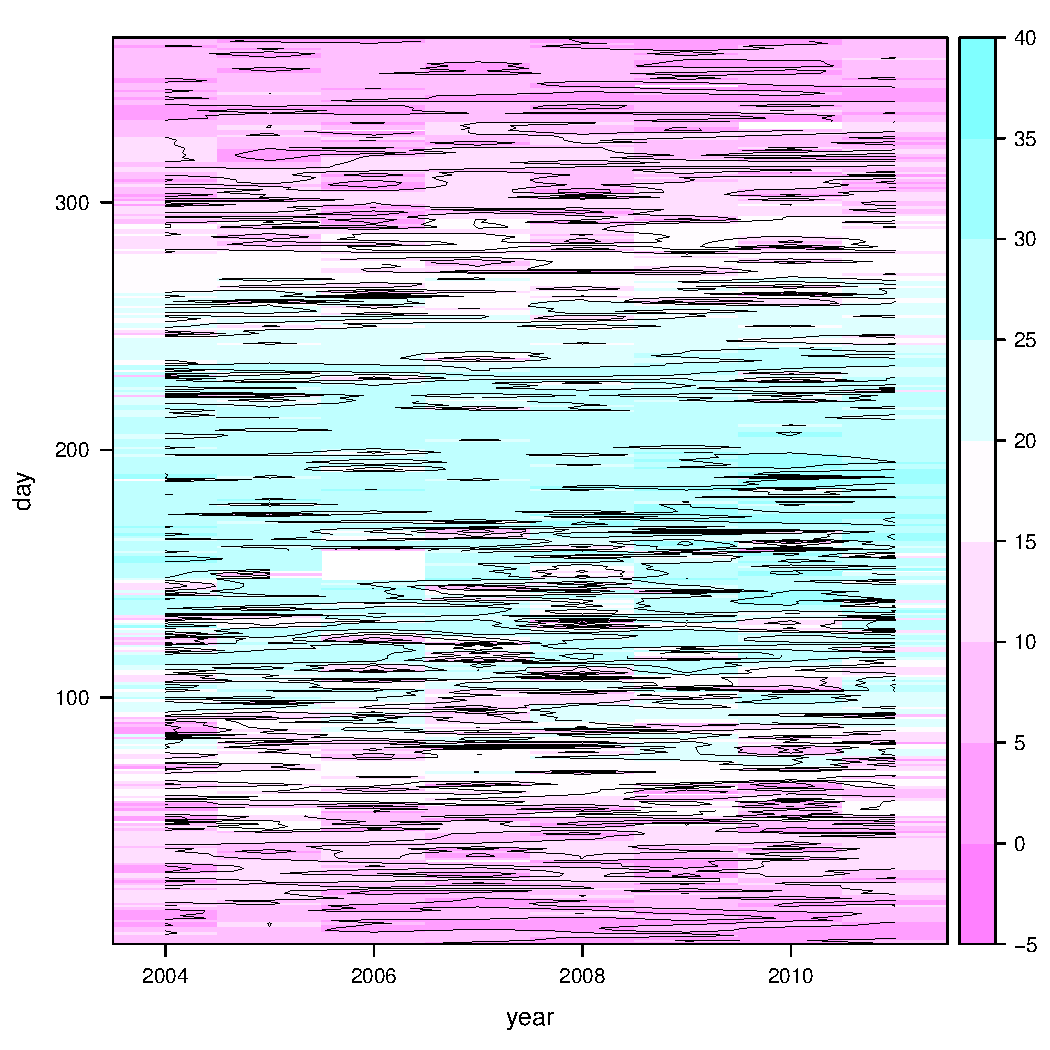
\includegraphics[width=.9\linewidth]{figs/contourplot.pdf}
\end{frame}
\begin{frame}[fragile,label=sec-2-1-20]{Box-and-Whiskers}
 \lstset{language=R,numbers=none}
\begin{lstlisting}
bwplot(Radiation ~ month, data=aranjuez,
       horizontal=FALSE, pch='|')
\end{lstlisting}

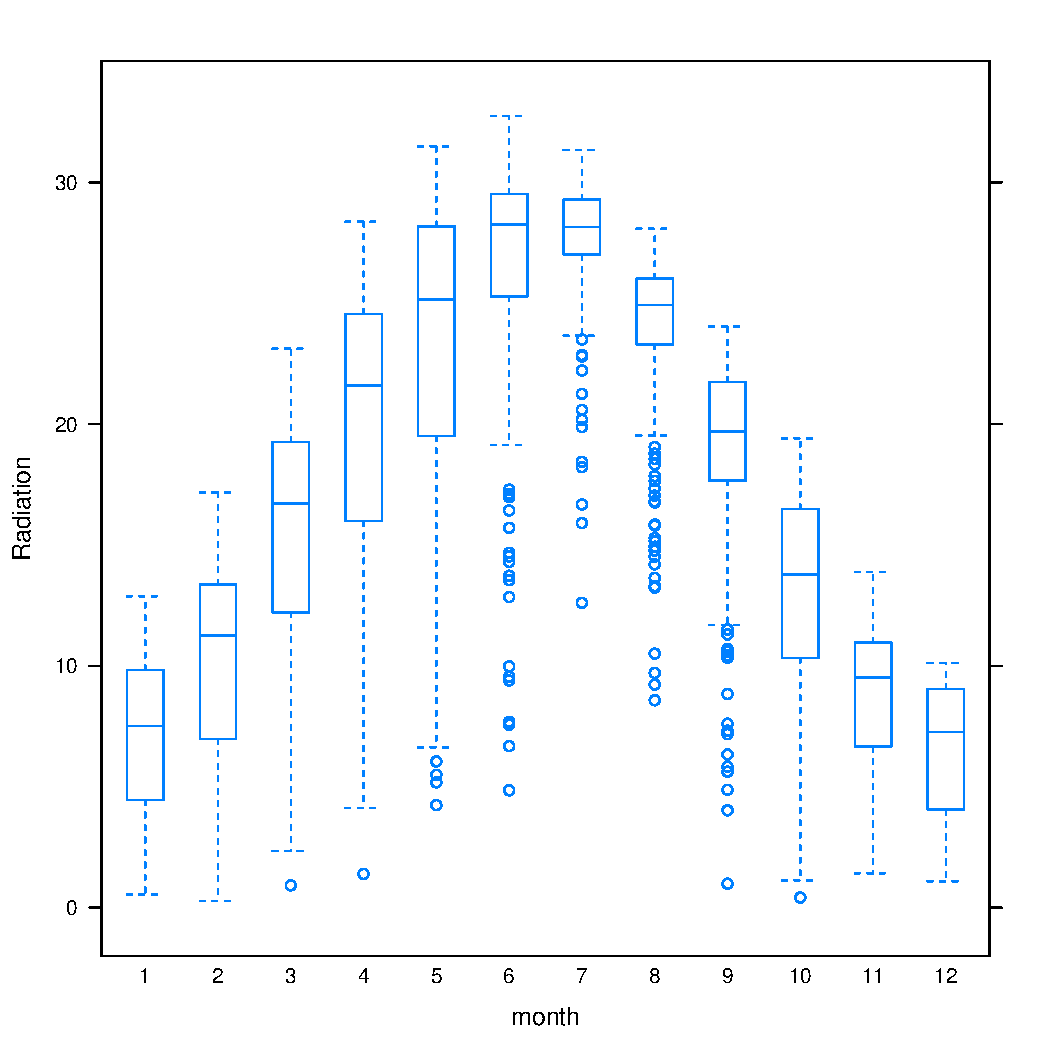
\includegraphics[width=.9\linewidth]{figs/bwplot.pdf}
\end{frame}
\begin{frame}[fragile,label=sec-2-1-21]{Box-and-Whiskers}
 \lstset{language=R,numbers=none}
\begin{lstlisting}
bwplot(Radiation ~ month, data=aranjuez,
       horizontal=FALSE,
       panel=panel.violin)
\end{lstlisting}

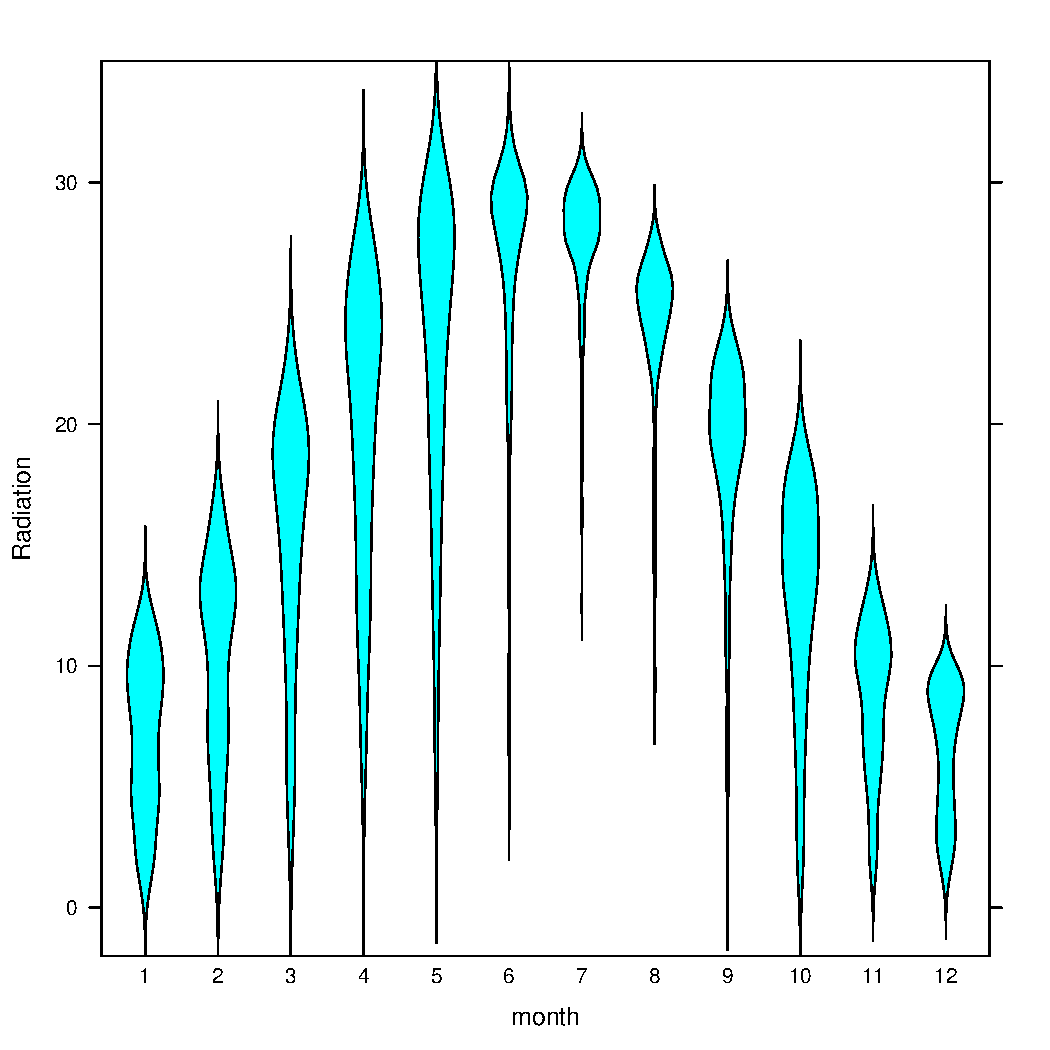
\includegraphics[width=.9\linewidth]{figs/violin.pdf}
\end{frame}

\begin{frame}[fragile,label=sec-2-1-22]{Histogramas}
 \lstset{language=R,numbers=none}
\begin{lstlisting}
histogram(~Radiation|factor(year), data=aranjuez)
\end{lstlisting}

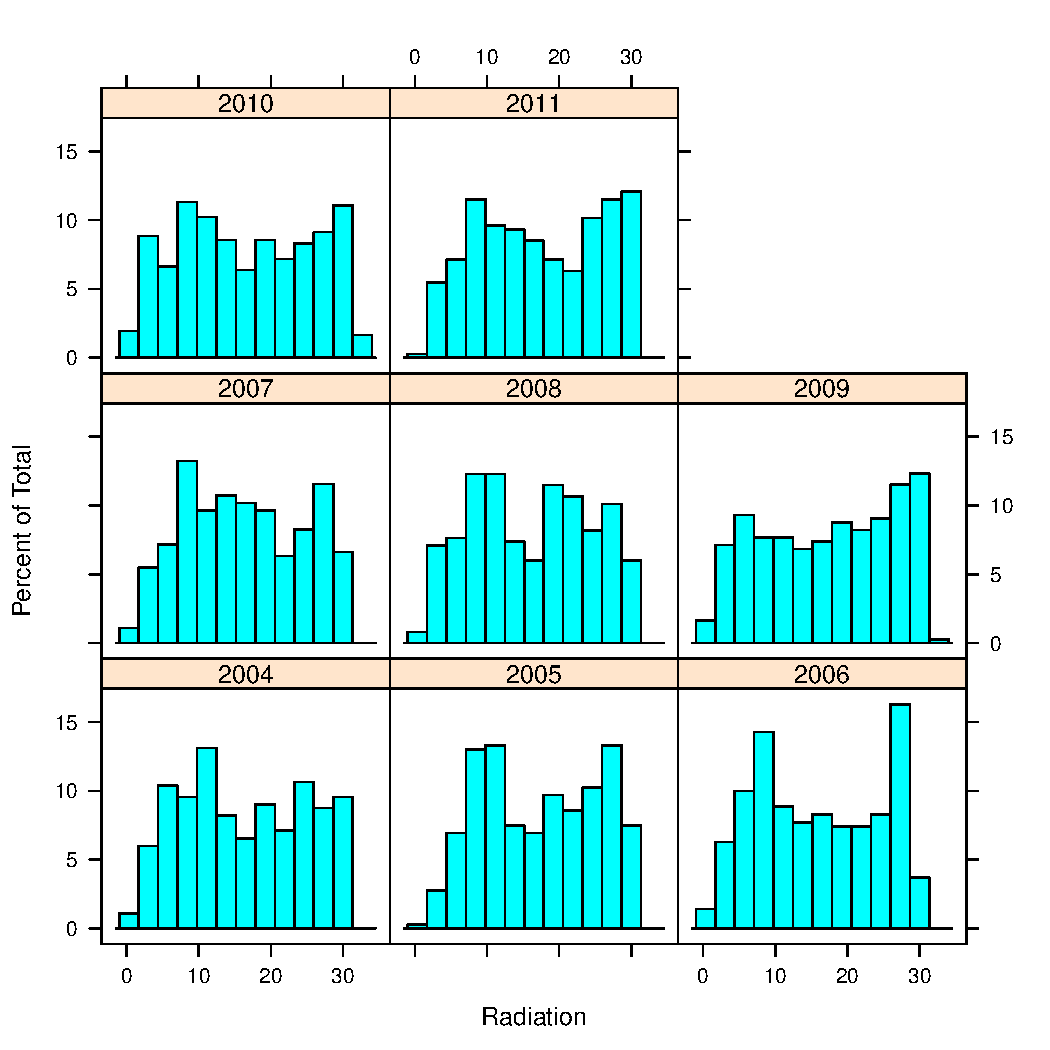
\includegraphics[width=.9\linewidth]{figs/histogram.pdf}
\end{frame}
\begin{frame}[fragile,label=sec-2-1-23]{Gráficos de densidad}
 \lstset{language=R,numbers=none}
\begin{lstlisting}
densityplot(~Radiation, groups=quarter,
	    data=aranjuez,
	    auto.key=list(space='right'))
\end{lstlisting}

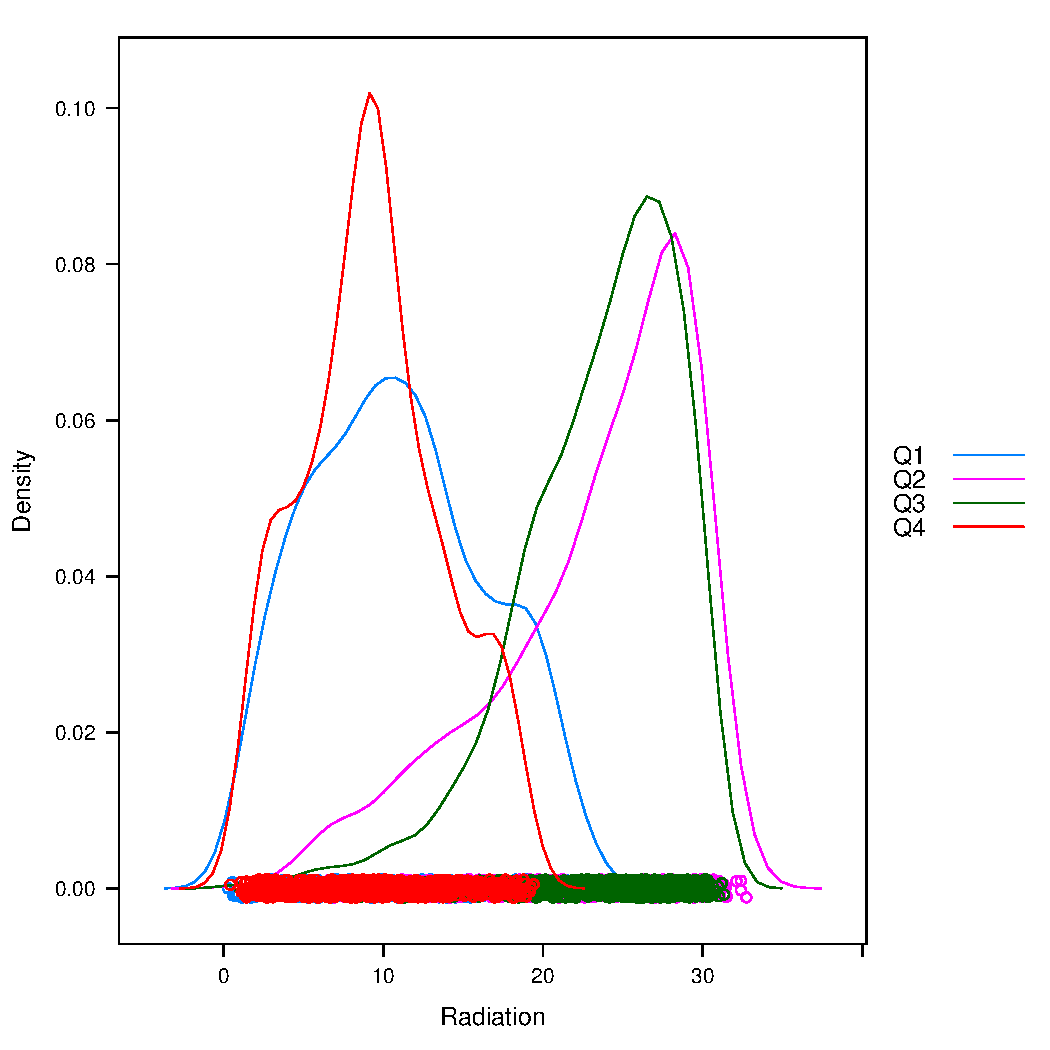
\includegraphics[width=.9\linewidth]{figs/density.pdf}
\end{frame}
\begin{frame}[fragile,label=sec-2-1-24]{\texttt{dotplot}}
 \lstset{language=R,numbers=none}
\begin{lstlisting}
avRad <- aggregate(Radiation ~ month * year,
		   data=aranjuez, FUN=mean)
\end{lstlisting}

\lstset{language=R,numbers=none}
\begin{lstlisting}
dotplot(month ~ Radiation|factor(year), data=avRad)
\end{lstlisting}

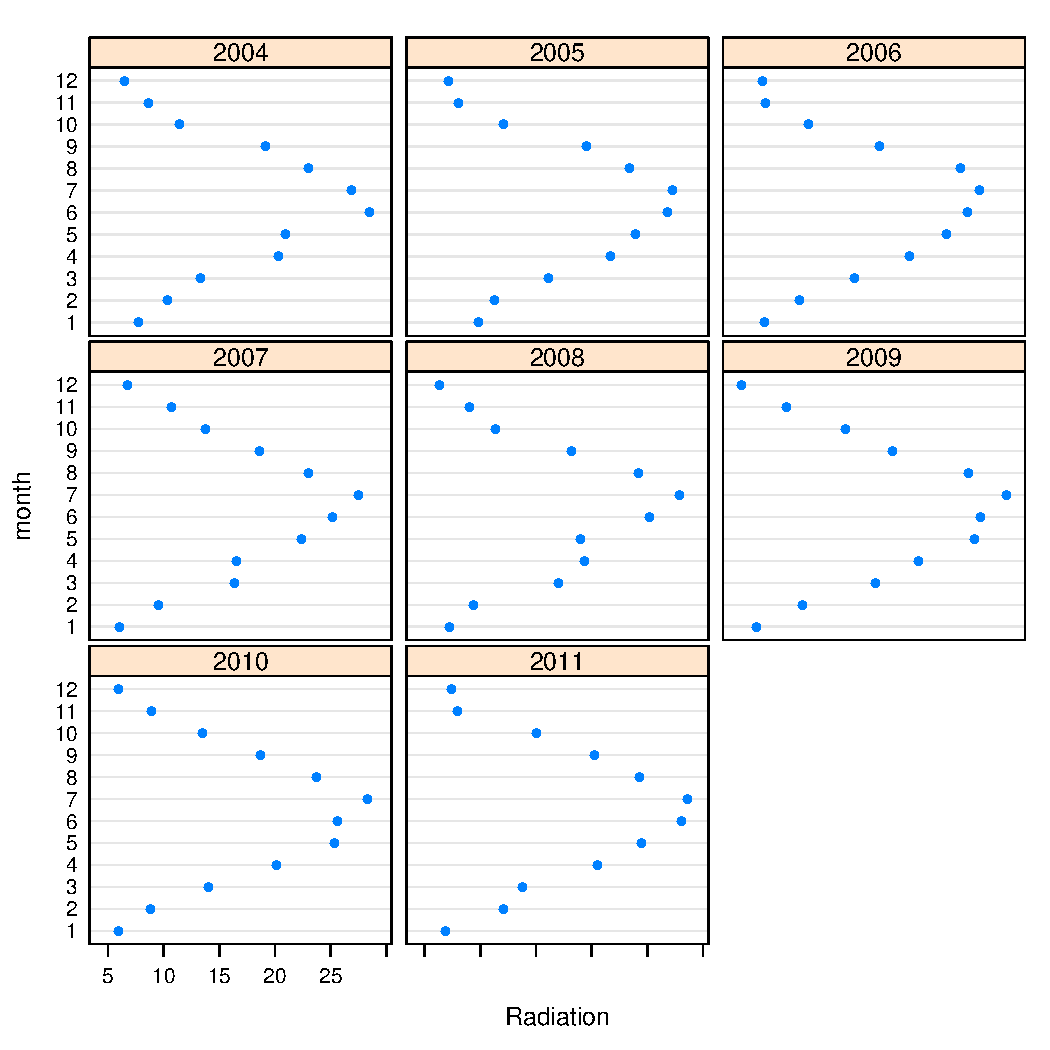
\includegraphics[width=.9\linewidth]{figs/dotplot.pdf}
\end{frame}

\begin{frame}[fragile,label=sec-2-1-25]{Quantile-Quantile}
 \lstset{language=R,numbers=none}
\begin{lstlisting}
firstHalf <- aranjuez$quarter %in% c('Q1', 'Q2')

qq(firstHalf ~ Radiation, data=aranjuez)
\end{lstlisting}

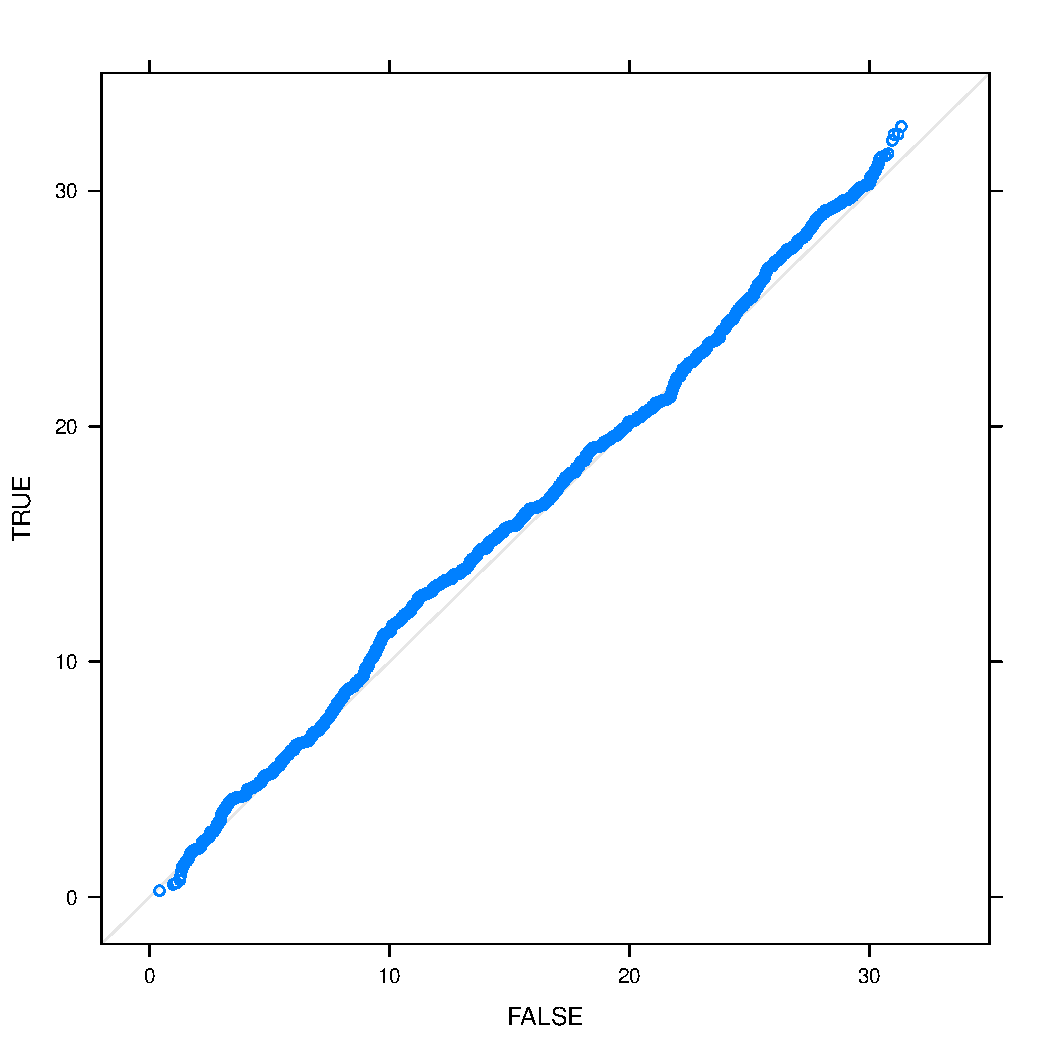
\includegraphics[width=.9\linewidth]{figs/qqHalf.pdf}
\end{frame}
\begin{frame}[fragile,label=sec-2-1-26]{Quantile-quantile}
 \lstset{language=R,numbers=none}
\begin{lstlisting}
winter <- aranjuez$quarter %in% c('Q1', 'Q4')

qq(winter ~ Radiation, data=aranjuez)
\end{lstlisting}

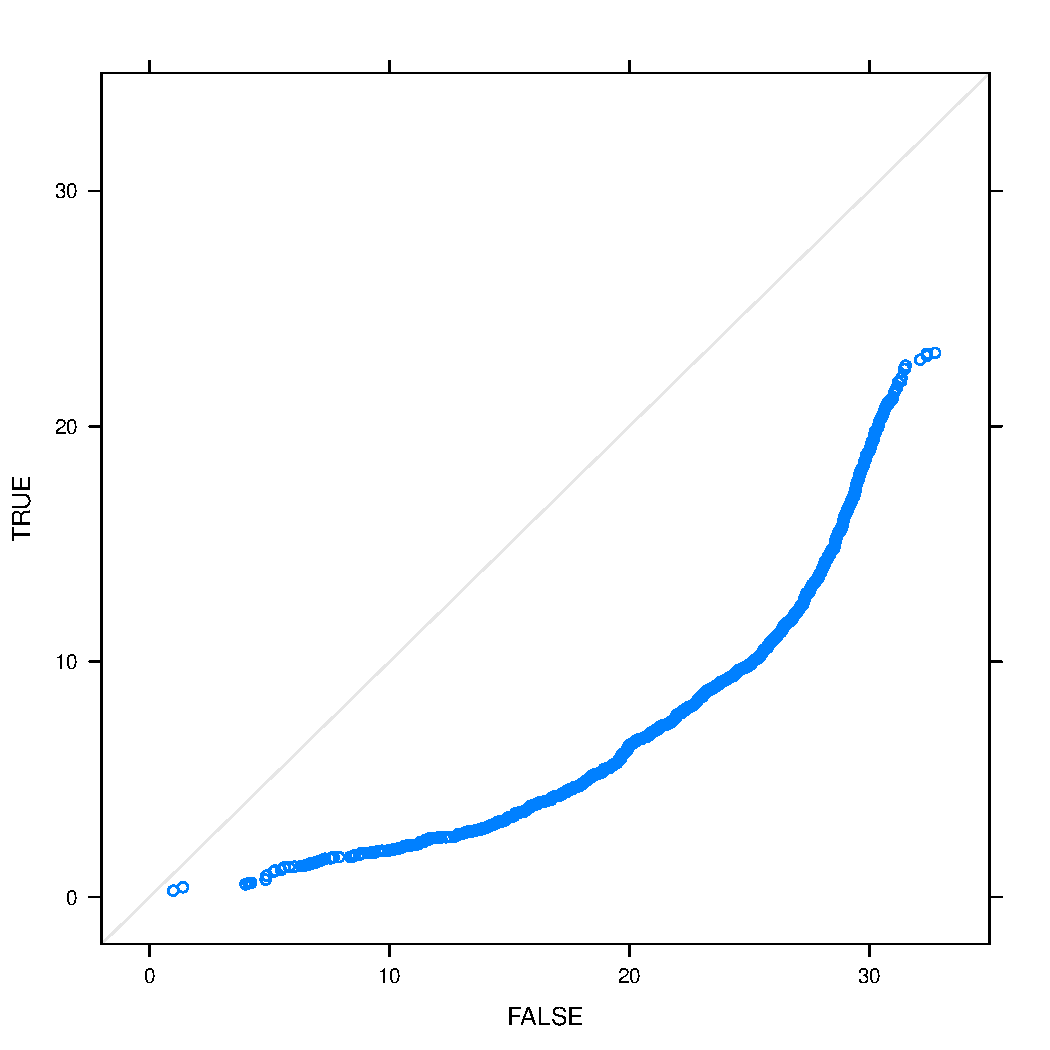
\includegraphics[width=.9\linewidth]{figs/qqWinter.pdf}
\end{frame}
\begin{frame}[fragile,label=sec-2-1-27]{Quantile-Quantile}
 \lstset{language=R,numbers=none}
\begin{lstlisting}
qqmath(~TempAvg, data=aranjuez,
       groups=year, distribution=qnorm)
\end{lstlisting}

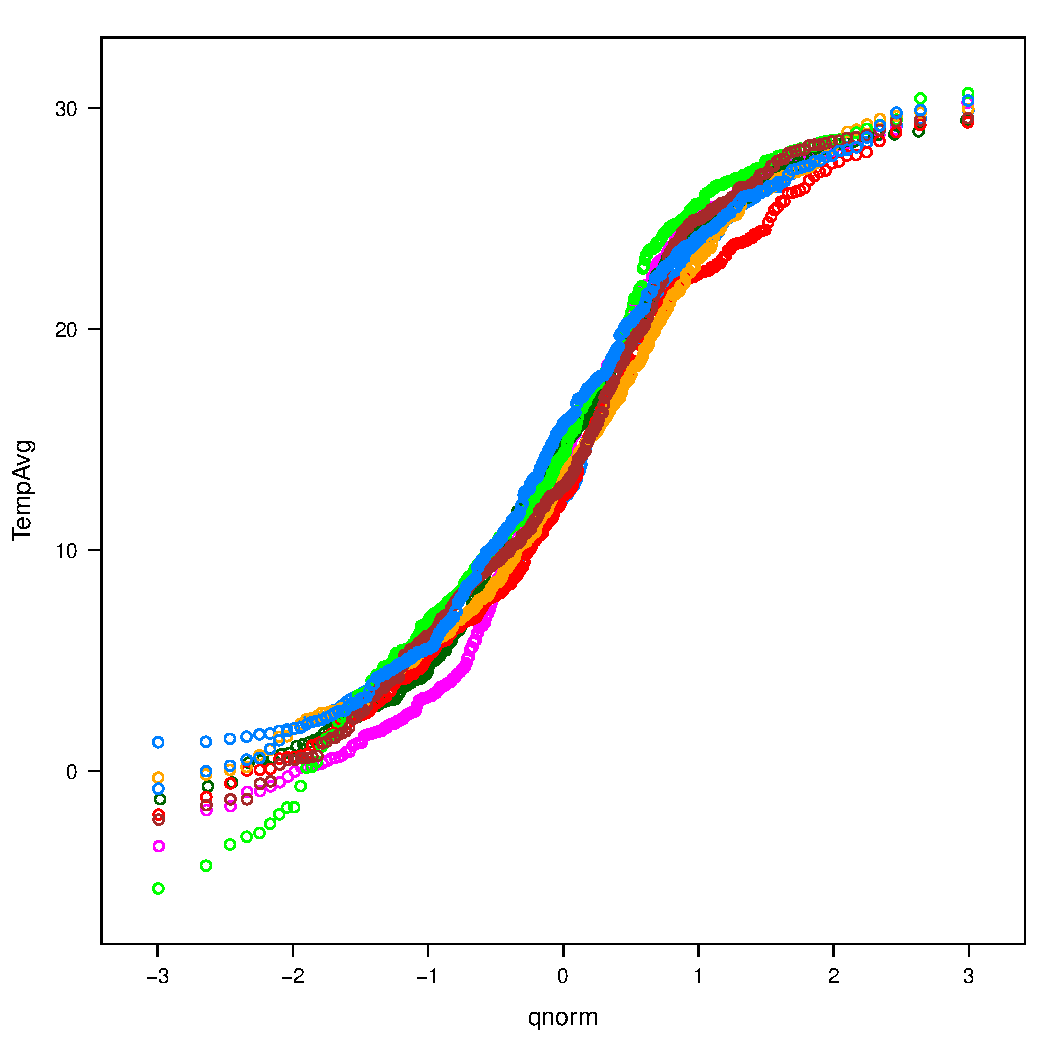
\includegraphics[width=.9\linewidth]{figs/qqNorm.pdf}
\end{frame}
\begin{frame}[fragile,label=sec-2-1-28]{Opciones de lattice}
 Todas las figuras han sido generadas con unas opciones previamente
definidas en \texttt{lattice.options}. Es necesario instalar el paquete
\texttt{latticeExtra}.
\lstset{language=R,numbers=none}
\begin{lstlisting}
library(latticeExtra)
myTheme=custom.theme.2(pch=19, cex=0.7,
		       region=rev(brewer.pal(9, 'YlOrRd')),
		       symbol = brewer.pal(n=8, name = "Dark2"))
myTheme$strip.background$col='transparent'
myTheme$strip.shingle$col='transparent'
myTheme$strip.border$col='transparent'
xscale.components.custom <- function(...){
    ans <- xscale.components.default(...)
    ans$top=FALSE
    ans}
yscale.components.custom <- function(...){
    ans <- yscale.components.default(...)
    ans$right=FALSE
    ans}
myArgs <- list(as.table=TRUE,
	       between=list(x=0.5, y=0.2),
	       xscale.components = xscale.components.custom,
	       yscale.components = yscale.components.custom)
defaultArgs <- lattice.options()$default.args
lattice.options(default.theme = myTheme, default.args = modifyList(defaultArgs, myArgs))
\end{lstlisting}
\end{frame}
\subsection{ggplot2}
\label{sec-2-2}

\begin{frame}[label=sec-2-2-1]{ggplot2}
\begin{itemize}
\item \href{http://docs.ggplot2.org/current/}{Documentación de ggplot2}
\item \href{http://ggplot2.org/book/}{Codigo del libro}
\item \href{http://learnr.wordpress.com/2009/06/28/ggplot2-version-of-figures-in-lattice-multivariate-data-visualization-with-r-part-1/}{ggplot2 desde lattice} (\href{http://learnr.files.wordpress.com/2009/08/latbook.pdf}{PDF})
\end{itemize}
\end{frame}
% Emacs 24.3.1 (Org mode 8.2.1)
\end{document}